%!TEX root = ../thesis.tex
%*******************************************************************************
%*********************************** First Chapter *****************************
%*******************************************************************************

\chapter{Introduction}  \label{c:1} %Title of the First Chapter 

\ifpdf
    \graphicspath{{Chapter1/Figs/Raster/}{Chapter1/Figs/PDF/}{Chapter1/Figs/}}
\else
    \graphicspath{{Chapter1/Figs/Vector/}{Chapter1/Figs/}}
\fi


%********************************** %First Section  **************************************
\section{The biology of ageing} %Section - 1.1 

\subsection{A brief introduction to ageing theory}

Potential quote: '... there are as many theories of ag[e]ing as there are biogerontologists.' Leonard Hayflick. Biological aging is no longer an unsolved problem

"At a fundamental level evolutionary survival is the preservation of a dynamic balance between information, or order, and entropy, or disorder." Thomas Kirkwood, Evolution of ageing, Nature 1977.

The ageing process is one of the most mysterious, complex and fascinating biological problems to be solved in the 21st century. Ageing and immortality have probably fascinated mankind since we have a conception of time and death \cite{Renfrew2016}. 

\bigskip

\textbf{Biological ageing} (aka the ageing process) can be broadly defined as the time-dependent functional decline which increases vulnerability to death in most organisms \cite{Lopez-Otin2013}. The revolution taking place in genetics and molecular biology during the 20th century gave rise to more than 300 theories that attempt to explain the mechanisms behind biological ageing \cite{Medvedev1990}. Any valid modern theory of ageing would need to explain at least two things \cite{Medvedev1990}:

\begin{itemize}
	
	\item The molecular causes behind the increase in \textbf{mortality rate} (aka death rate) over time in a given species population. Mortality rate can be broadly defined as the number of deaths in a population per unit of time and scaled by the size of the population. More formally, by quantifying the deaths of individuals in a population over time (and assuming that there are no increases in the population number due to reproduction, migration, ...), the survival fraction at a given time $t$, $S(t)$, is \cite{Witten1986}:
	
	\begin{align}
	S(t) = \frac{N(t)}{N_0}
	\end{align}
	
	where $N(t)$ is the number of individuals alive at a given time $t$ and $N_0$ is the initial number of individuals in the population. It can be demonstrated that the mortality rate, $\lambda(t)$, can be expressed as \cite{Witten1986}:
	
	\begin{align} \label{eq:1.2}
	\lambda(t) = - \frac{1}{S(t)} \cdot \frac{dS(t)}{dt}
	\end{align}
	
	\item The \textbf{evolutionary variations in lifespan between different species} \cite{Jones2013}; where lifespan is defined as the time passed between birth and death of an organism. For example, the maximum lifespan in the case of the roundworm (\textit{Caenorhabditis elegans}) is 0.16 years (58.4 days, in captivity); in the case of the fruit fly (\textit{Drosophila melanogaster}) is 0.3 years (109.5 days, in captivity); in the case of the house mouse (\textit{Mus musculus}) is 4 years (in captivity); in the case of humans (\textit{Homo sapiens}) is 122.5 years and in the case of the bowhead whale (\textit{Balaena mysticetus}) is 211 years (in the wild) according to the database AnAge \cite{DEMAGALHAES2009}. Furthermore, some species (such as certain turtles, certain species of rockfish or the bristlecone pine) seem to have negligible senescence i.e. negligible changes in adult mortality rates over extended periods of time at advanced adult ages \cite{Finch2009}.   
	
\end{itemize}

Nowadays, there are at least \textbf{two main paradigms}, complementary to each other, that try to conceptualise the problem and that are a topic of intense discussion among gerontologists:

\begin{itemize}
	
	\item Ageing as a consequence of \textit{molecular infidelity}. In this case, stochastic chemical modifications of biomolecules, such as DNA or proteins, exceed the capacity of the repair and turnover systems of the organism and accumulate over time, which increases the entropy of the system. This leads to changes in molecular structure and, finally, changes in function, which increase vulnerability to age-related diseases \cite{Hayflick2007,Hayflick2007a}. From an evolutionary point of view, this fits into the \textit{disposable soma theory}, originally proposed by Thomas Kirkwood in 1977. This theory suggests that organisms have evolved to optimise the amount of energy dedicated to repair errors in somatic cells in order to maximise reproductive success (at the expense of indefinite survival) \cite{Kirkwood1977,Kirkwood1991}. 
	
	\item Ageing as a consequence of \textit{hyperfunction}. In this case, the primary cause of ageing is an excessive activity of certain growth or development-related genes and pathways in later life \cite{Blagosklonny2006,Blagosklonny2010,DeMagalhaes2012,Gems2015}. In other words, ageing would be a program for development that has not been turned off \cite{Blagosklonny2006}. This idea is rooted on the concept of \textit{antagonistic pleiotropy}, an important pillar of the evolutionary theory of ageing originally proposed by George C. Williams in 1957 \cite{Williams1957}. It implies that certain genes have opposite effects on fitness at different ages, which is a consequence of the decrease in selection forces after reproductive age. A strong candidate is the \acrshort{TOR} (target of rapamycin) pathway, which promotes development in early life but also the advancement of several late-life pathologies \cite{Blagosklonny2010}. 
	
\end{itemize}

It has become clear that no single molecular mechanism will be able to explain ageing across all kingdoms of life. Different species have different life histories that are subjected to evolutionary trade-offs (e.g. regarding reproduction strategies, developmental schedules, ...) and that can affect the rate of ageing \cite{Ricklefs2010,Jones2013}. Nevertheless, it is possible to integrate all the ideas presented so far into a \textbf{theoretical framework} that can help to unify definitions across studies and set the foundations for mechanistic advancements on the biology of ageing (Fig.~\ref{fig:c1_fig1}, inspired by ideas from \cite{Hayflick2007,Gems2015,Peto1997,Freund2019}). Under this theoretical framework: 

\begin{itemize}
	
	\item The ageing process is composed of different molecular mechanisms (subprocesses) that are operative at different stages of life and contribute, in variable proportions, to the appearance of different age-related diseases i.e. the risk of developing an age-related disease is the `integral of its ageing subprocesses operating over time'. Furthermore, the development of different diseases affects the mortality rate and, thus, the probability to die. The different ageing processes can also be understood as the sources of ageing-causing molecular damage \cite{Lopez-Otin2013}.
	
	\item If the ageing subprocesses can be altered through different genetic, lifestyle of pharmacological interventions, it is possible to reduce the likelihood of several age-related diseases at the same time. This makes ageing research incredibly relevant for the biomedical sciences, since it changes the current paradigm of developing interventions for a specific already-existing disease towards the prevention of several diseases simultaneously.
	
	\item  Differences in the average lifespan between different species should be explained by different combinations of ageing subprocesses and their rates.
		
\end{itemize}	

Consequently, systems biology approaches become fundamental to understand the ageing process \cite{Freund2019}. In the next sections, I will provide an overview of the ageing mechanisms that may be operative in different species, with a special focus on mammalian species. 

\begin{figure}[htbp!] 
	\centering    
	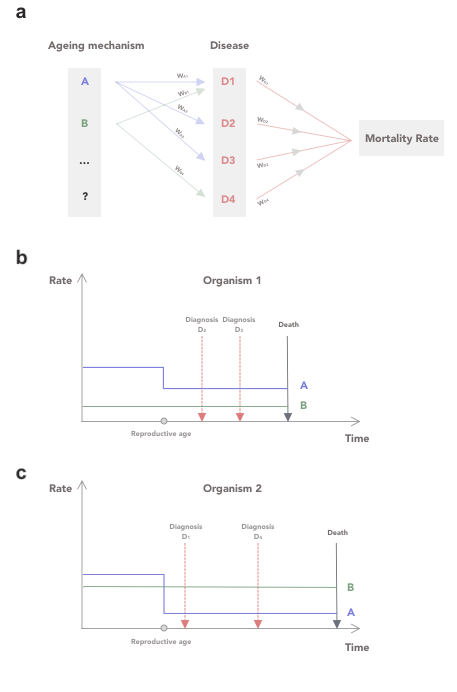
\includegraphics[width=0.8\textwidth]{C1_Fig1}
	\vspace*{1 mm}
	\caption[Theoretical framework to conceptualise the ageing process]{Theoretical framework to conceptualise the ageing process. \textbf{a.} The ageing process is composed of different molecular mechanisms (subprocesses) that are operative at different stages of life and contribute, in variable proportions (specified by the weights), to the appearance of different age-related diseases. Furthermore, the development of different diseases affects the mortality rate and, thus, the probability to die. \textbf{b.} and \textbf{c.} Examples of the life histories of two organisms. In these examples, two ageing mechanisms are operative: A (which changes its rate after reproductive age e.g. activated growth-related pathways) and B (with a constant rate over time e.g. some type of (epi)mutational process). Differences in the mechanisms' profiles lead to differences in the age-related diseases that manifest over the lifespan of the organisms, even though the molecular mechanisms are the same. This, affects the mortality rate and, ultimately, the time-to-death. This figure is inspired by ideas from \cite{Hayflick2007,Gems2015,Peto1997,Freund2019}.}
	\label{fig:c1_fig1}
\end{figure}

\smallskip

\subsection{The genetic basis of ageing} \label{s:1.1.2}

\smallskip

Given the differences in the lifespan between species and even within species \cite{Jones2013, Gems2000}, it is nowadays clear that the ageing process must have a genetic basis. However, for a long time, the ageing process was thought to be a `haphazard process driven solely by entropy' \cite{Kenyon2005}. Furthermore, in 1935 Clive Maine McCay had shown that caloric restriction (a reduction in calories intake without malnutrition) could extend mean and maximal lifespan in rats \cite{McCay1935,McDonald2010}, which probably shifted the focus towards environmental or external causes as the main driver forces of the ageing process. Since then, dietary restriction (different types of dietary interventions that reduce food intake without malnutrition) has been established as the most successful non-genetic intervention to slow down the ageing process across species \cite{Fontana2015}.

\bigskip

The establishment of the nematode \textit{Caenorhabditis elegans} as a model organism in the 70s triggered its adoption in the ageing field \cite{KLASS1976}, since it allowed well-controlled experiments in a much shorter period of time than rodents \cite{Johnson2013}. This lead to the discovery of the first mutants that dramatically extended lifespan, which mapped to genes in the insulin/IGF-1 signalling pathway \cite{Kenyon1993,Morris1996}. Since then, many genes have been found to significantly affect the lifespan of other model organisms as well, such as budding yeast (\textit{Saccharomyces cerevisiae}), fruit fly (\textit{Drosophila melanogaster}) or mouse (\textit{Mus musculus}) \cite{Kenyon2005,Kenyon2010,Singh2019}. 

\bigskip

Interestingly, the effects of many of these genetic mutations and their pathways are shared by distantly-related species. This suggests that at least part of the molecular mechanisms that drive the ageing process could be evolutionarily conserved. Among these ageing-related signalling pathways it is worth highlighting (Fig.~) \cite{Kenyon2005,Kenyon2010,Singh2019,Greer2008}:

\begin{itemize} 

	\item \textbf{Insulin/\acrshort{IGF-1} pathway}. This underscores the central role of the endocrine system on the biology of ageing. Mutations that lower the level of \textit{daf-2}, encoding an insulin/IGF-1 receptor, were originally found to double the lifespan of \textit{C. elegans} \cite{Kenyon1993,Guarente2000}. Activation of the insulin/IGF-1 pathway, a PI3K pathway, leads to the phosphorylation of a transcription factor of the FOXO family, encoded by \textit{daf-16} in \textit{C. elegans}, which prevents it to reach the nucleus \cite{Lin2001}. FOXO transcription factors, of which there are several members in mammals, activate the expression of longevity-promoting genes involved in processes such as autophagy (which clears protein aggregates and damaged organelles in the cell) \cite{Singh2019}, resistance to oxidative stress or stem cell maintenance \cite{Martins2016}. This partially explains why inhibiting the insulin/IGF-1 pathway can increase organismal lifespan. However, other downstream targets that regulate gene expression have been identified, such as \textit{hsf-1} (a transcription factor that regulates heat-shock response) \cite{Hsu2003} or \textit{skn-1} (a transcription factor that coordinates a response to oxidative stress) \cite{Tullet2008} in \textit{C. elegans}.
	
	\item \textbf{\acrshort{TOR} pathway}. \acrshort{TOR} (target of rapamycin) is a kinase that acts as a major amino-acid and nutrient sensor by stimulating growth (including protein translation) and blocking autophagy \cite{Kenyon2010}. The effects of TOR are partly mediated by activating the ribosomal subunit S6 kinase (which promotes protein translation) and by inhibiting 4EBP (a translation inhibitor)  \cite{Kenyon2010,Um2006}. Reductions in TOR activity (through mutation, downregulation or pharmacologically) increase lifespan across many species \cite{Kenyon2010}. Importantly, rapamycin, a drug that inhibits TOR, can increase the mean lifespan of mice when fed late in life, which showed for the first time that pharmacological interventions of mammalian ageing are possible \cite{Harrison2009}. Interestingly, the increase in lifespan differed in males (9\%) and females (13\%) \cite{Harrison2009}, highlighting the sex-specific effects of some ageing mechanisms. 
	
	\item \textbf{AMPK pathway}. The AMP-activated kinase (\acrshort{AMPK}) controls the balance between catabolic and anabolic processes depending on the cellular levels of \acrshort{AMP}/\acrshort{ATP} (i.e. when ATP levels decrease, AMPK is activate to promote catabolic pathways) \cite{Kenyon2010,Mihaylova2011}. Furthermore, AMPK activation promotes autophagy, partially by inhibiting TOR \cite{Mihaylova2011}.The anti-diabetic drug metformin, which activates AMPK among other targets, has been shown to extend lifespan in mice \cite{Anisimov2008,Martin-Montalvo2013} and has currently been included as the first drug to target the human ageing process in a clinical trial \cite{Barzilai2016}.
		
	\item \textbf{Sirtuins}. Sirtuins are a family of nicotinamide adenine dinucleotide (\acrshort{NAD$^+$})-dependent deacetylases i.e. they generally catalyse the removal of an acetyl group from lysine residues using \acrshort{NAD$^+$} as a cofactor \cite{Bonkowski2016}. Sirtuins have been shown to play complex roles in the biology of ageing and age-related diseases, in general by cross-talking with other nutrient-sensing pathways and promoting longevity \cite{Kenyon2010,Bonkowski2016}. Several authors have shown that increasing \acrshort{NAD$^+$} levels enhances the activity of sirtuins, which could constitute an additional anti-ageing pharmacological avenue in mammals. Additionally, intensive research is being carried out to identify other molecules that activate sirtuins \cite{Bonkowski2016}.
	
	\item \textbf{Other pathways}. Mitochondrial respiration (and its association with reactive oxigen species or \acrshort{ROS}), genome surveillance pathways (such as those involved in DNA repair or telomere maintenance), signals from the reproductive system or Wnt signalling have also been implicated in different ways in the ageing process \cite{Kenyon2010,Greer2008, Lezzerini2014}.
	
\end{itemize}

\bigskip

These pathways seem to have a dual role depending on the environmental context that the organism is facing, behaving as \textbf{nutrient and stress sensors} (Fig.~). Under abundant nutrient availability and low stress (oxidative, temperature), they tend to promote growth and reproduction. On the contrary, under harsh conditions (such as those posed by dietary restriction), they favour cell protection and maintenance \cite{Kenyon2005,Kenyon2010}. It is worth mentioning that the responses of the different pathways to dietary restriction deeply depend on the characteristics of the diet and its timing \cite{Kenyon2010}. This model also relates to the disposable soma theory, where more resources are allocated either to reproduction or somatic maintenance depending on the context \cite{Kirkwood1977,Kirkwood1991}. This is further mechanistically supported by experiments that show that decreased insulin/IGF-1 signalling (e.g. via \textit{daf-2} mutation) produces the acquisition of germline characteristics (e.g. higher genomic stability) in \textit{C. elegans} \cite{Curran2009}. Even though this model is a clear oversimplification, it becomes useful when thinking about the way that the ageing process might have evolved and how the same biological pathways can be repurposed to activate complex genetic programs with completely different goals.

\bigskip

There are many more \textbf{complexities associated with these pathways} that would require an entire thesis in its own. For example, the insulin/IGF-1 signalling pathway can work in a cell non-autonomous manner (i.e. the activity of the pathway in one tissue can affect lifespan by influencing cells in a different tissue), which could help to coordinate ageing rates in the organism, and the effects are many times tissue-specific \cite{Kenyon2005,Kenyon2010}. Additionally, the pathways can have different effects depending on the life stage of the animal (e.g. development, adulthood, ...) \cite{Dillin2002}. Furthermore, cross-talk between the pathways has previously been reported \cite{Bonkowski2016, Greer2007}. Therefore, the inner workings of these signalling pathways is still a topic of intense research.

\bigskip

The discovery of genetic pathways that can dramatically extend the lifespan of model organisms has demonstrated that \textbf{the ageing process has a genetic basis and it is possible to alter its rate}. More importantly, the appearance of age-related disease seems to be delayed in many of these long-lived organisms \cite{Kenyon2010,Arantes-Oliveira2003}, suggesting that these interventions indeed reduce the rate of some the operating ageing mechanisms (Fig.~\ref{fig:c1_fig1}) and opening the door to the development of anti-ageing interventions. 

\smallskip

\subsection{Hallmarks of mammalian ageing} \label{s:1.1.3}

\smallskip

Most mammalian studies on the biology of ageing have been conducted in the mouse. Many genetic mutations in conserved pathways (mainly nutrient-sensing pathways) have been shown to significantly extend the lifespan of mice. Among them, those that affect growth hormone signalling, which in mammals in turn controls the secretion of IGF-1 by the liver and therefore the insulin/IGF-1 signalling pathway, produce the longest lifespan improvements (in the order of 40-60\%) \cite{Singh2019}. Even though this is a remarkable result, it is far off the lifespan extensions achieved with `simpler' model organisms such as \textit{C. elegans} (where extensions of almost 1000\% have been achieved with a mutation in a single gene of the insulin/IGF-1 pathway; the equivalent of a human living up to $\approx 1200$ years!) \cite{Ayyadevara2008}. This highlights a trend where translating lifespan interventions discovered in worms and flies yields generally less spectacular results in mice and potentially humans.

\bigskip

Evolution has been experimenting with lifespan extension for a long time. Consequently, some species of mammals, such as the naked mole rat (\textit{Heterocephalus glaber}) or some species of bats, are exceptionally long-lived for their body size. Recent reports point towards the possibility that these species do not increase their mortality rate with age (i.e. they have negligible senescence) \cite{Ruby2018,Fleischer2017}, which makes them incredibly interesting systems to study the biology of ageing in mammals. 

\bigskip

In 2013, L\'opez-Ot\'in \textit{et al.} reviewed the main common denominators of the ageing process across organisms \cite{Lopez-Otin2013}. They defined several \textbf{hallmarks of ageing}, which can be understood as the measurable consequences of the ageing mechanisms that I proposed in Fig~\ref{fig:c1_fig1}. I will briefly discuss some of them, with a special focus on those that directly affect the genome during mammalian ageing  \cite{Lopez-Otin2013,Singh2019}:

\begin{itemize}
	
	\item \textbf{Genomic instability}. Somatic DNA mutations (single nucleotide variants, copy number changes, structural rearrangements, ...) accumulate over time in the genomes of mammalian cells (both in the nuclear genome and the mitochondrial genome) \cite{Martincorena2018,Larsson2010}. Different mutational processes (good candidates for ageing mechanisms) create specific patterns of mutations (aka mutational signatures) in the genome, which have been widely studied in the context of human cancer \cite{Alexandrov2014}. It is possible to assign specific endogenous (e.g. DNA replication errors) and exogenous factors (e.g. smoke exposure) that contribute to the different processes. In the context of ageing, deamination of 5-methylcytosine (\acrshort{5mC}) in a \acrshort{CpG} context leads to C>T (cytosine to thymine) mutations, which accumulate in a clock-like manner with a rate that seems to correlate with the proliferative activity of the tissue \cite{Alexandrov2015}. Furthermore, nuclear architecture and the 3-dimensional organisation of the genome both seem to change with age, which can distort nuclear homeostasis. Interestingly, several human diseases that are considered to display premature ageing, such as Werner syndrome or Hutchinson–Gilford progeria, have mutations in proteins that lead to genomic instability \cite{Oberdoerffer2007}. Finally, it is possible that an increase in the mobilisation of transposable elements with age further contributes to destabilise the genome \cite{Orr2016}.
	
	\item \textbf{Telomere attrition}. The repetitive DNA linear ends of mammalian chromosomes are capped with a protein complex (shelterin) to form structures known as telomeres. Due to the nature of the standard DNA replication machinery, the chromosomal DNA ends of somatic cells are eroded after each cell division (net loss of 100-200 bp of telomeric sequence per cell division). After a certain number of doublings (and therefore telomeres shortening) cells stop diving and they induce cellular senescence (see below) or cell death (apoptosis) \cite{OSullivan2010}. For many years, this replicative limit, known as the Hayflick limit, was understood as the manifestation of the ageing process at the cellular level \cite{Hayflick1961,Hayflick1998}. Telomere shortening has indeed been shown to occur with age in most humans tissues \cite{Blasco2007}. Importantly, stem cells and germ cells express telomerase, an enzymatic complex that synthesises new telomeric repeats, avoiding telomere shortening. This way organisms can regenerate their tissues if needed, which makes it unlikely that telomere attrition is the only mechanism behind ageing. Furthermore, in mammals other mechanisms could contribute to replicative senescence besides telomere length \cite{OSullivan2010}. Nevertheless, telomere biology plays a critical role in many fundamental processes, such as DNA repair and genomic stability, and non-telomeric functions for telomerase have also been suggested (such as global chromatin regulation and transcription of developmentally-regulated genes) \cite{OSullivan2010}. As such, telomere biology has been implicated in age-related diseases, such as cancer and cardiovascular disease \cite{OSullivan2010,Blasco2007}. Interestingly, ectopic expression of the catalytic subunit of telomerase (TERT) extends the lifespan of mice that are cancer-resistant \cite{Tomas-Loba2008}. 
	
	\item \textbf{Epigenetic alterations}. This hallmark is reviewed in further detail in section~, since it is the main focus of this thesis.
	
	\item \textbf{Cellular senescence}. Cellular senescence is a cellular state characterised by a stable cell cycle arrest. There are different types of senescence induced by different stress stimuli, including telomere shortening (replicative senescence, previously mentioned), sustained DNA damage (e.g. via irradiation) or derepression of the \textit{INK4/ARF} locus (which encodes three tumour suppressor genes)\cite{Lopez-Otin2013,Herranz2018}. Under normal circumstances, cellular senescence carries out physiological functions such as stopping pre-malignant cells from dividing, wound healing and tissue remodelling. Furthermore, senescent cells also secrete a cocktail of factors (termed the senescence-associated secretory phenotype, or \acrshort{SASP}) with pleiotropic effects (pro-inflammatory, matrix remodelling, inducing growth, ...) \cite{Herranz2018}. Senescent cells seem to accumulate in some mammalian tissues during ageing. If this happens in excess, the SASP can perturb the homeostasis of the tissue. Consequently, the removal of senescent cells in mice increases lifespan and reduces the appearance of age-related phenotypes \cite{Baker2011,Baker2016,Xu2018}. Drugs that selectively induce apoptosis in senescent cells (known as senolytics) \cite{Kirkland2017} are currently undergoing clinical trials in humans. 
	
	\item \textbf{Other hallmarks of ageing}. These include loss of proteostasis (appropriate quality control of the proteome, which is mechanistically connected with autophagy pathways; strongly implicated in neurodegenerative diseases); deregulated nutrient sensing (mediated by the pathways discussed in section~\ref{s:1.1.2}; it is important to mention that in mammals the insulin/IGF-1 pathway is integrated in the somatotrophic axis, which involves the growth hormone as an activator of IGF-1 production and ); mitochondrial dysfunction (including a reduction in the efficacy of the respiratory chain with age); stem cell exhaustion (which is thought to contribute to the decline of regenerative potential of the tissues with ageing, such as in the case of the haematopoietic system) and altered intercellular communication (including an increase in inflammation, known as inflammageing, or alterations in the neuroendocrine system) \cite{Lopez-Otin2013}.

	
\end{itemize}

Importantly, complex interactions and interdependencies emerge between the different hallmarks of ageing. For example, in senescent cells in the mouse, a type of transposable element (L1) becomes derepressed and activates type-I interferon response, which in turn causes inflammageing \cite{DeCecco2019}. Furthermore, understanding the role of the environment in modulating the ageing process and the different hallmarks in mammals is becoming increasingly important.  

\bigskip

Assuming that molecular damage is the main cause of biological ageing, the mechanisms that lead to genomic instability, telomere attrition, epigenetic alterations and loss of proteostasis are very likely the main drivers of the ageing process, with the rest of the hallmarks being a consequence of them \cite{Lopez-Otin2013}. Nevertheless, interventions targeting some of the more `integrative hallmarks' (such as removing senescent cells, optimising dietary restriction or stem cell therapies) will probably arrive earlier in the clinic.

\smallskip

\subsection{Studying the ageing process in humans}

\smallskip

Average human lifespan has nearly doubled in most developed countries during the last 200 years. This has been the consequence of external factors, such as improvements in quality of water, food, hygiene, housing and lifestyle, immunization against infectious disease, antibiotics and medical care \cite{Partridge2018}. One of the most debated questions in the human ageing field is whether there is a limit to maximal human lifespan \cite{Dong2016}. Since Benjamin Gompertz's pioneering work in 1825, it is known that the mortality rate in humans increases exponentially with age \cite{Gompertz1825}. However, a recent study on Italian centenarians suggests that mortality rate, which increases exponentially up to about age 80, decelerates thereafter and reaches or closely approaches a plateau after age 105 \cite{Barbi2018}. This implies that human lifespan will likely continue to increase in the next decades and that \textbf{we have probably not reached our lifespan evolutionary limit as a species yet} \cite{Barbi2018,Kontis2017}. 

\bigskip

Thus, in order to avoid a massive socioeconomic burden on our societies \cite{Fine2014}, biomedical research should focus on \textbf{extending human healthspan} (i.e. the amount of time that we live free of disease) and not only lifespan. This goal, known as the `compression of morbidity' \cite{Partridge2018}, is theoretically possible if we target the core mechanisms that drive the ageing process (Fig~\ref{fig:c1_fig1}), which is assumed to be the biggest contributor to the development of most age-related diseases, such as cancer, diabetes, cardiovascular disorders and neurodegenerative diseases \cite{Lopez-Otin2013}. Indeed, genetic and pharmacological interventions that increase lifespan in model organisms also seem to extend healthspan \cite{NewellStamper2018} and the compression of morbidity is a characteristic of human centenarians \cite{Feldman2012}.  

\bigskip

Most of our understanding of human ageing comes from studies carried out in \textbf{population cohorts}. Furthermore, during the last years different datasets of high-throughput molecular data (broadly know as `omics') have been generated for many of these cohorts, including genetic data, epigenetic data, metabolomic data, imaging data or even the microbiome. These data (sometimes referred as `deep phenotypes') complement the more traditional phenotypic measurements and health records and allow, for the first time, characterising the human ageing process with unprecedented resolution and scale. An example of such a cohort is the UK Biobank, which has enrolled > 500,000 participants \cite{Bahcall2018}. Importantly, there is a trend in many of these cohorts to collect more longitudinal data (i.e. data over time for the same individual), which will likely increase the power to discover causal ageing mechanisms when compared with cross-sectional data (i.e. when data from different individuals at different ages is used) \cite{Rahmadi2017}. As Nobel laureate Sydney Brenner (known for establishing \textit{C. elegans} as a model organism) remarked 10 years: "We don't have to search for a model organism anymore. Because we are the model organisms" \cite{FitzGerald2018} (as a disclosure, I still believe we need model organisms to gain definitive mechanistic insights, and probably so does Dr. Brenner). 

\bigskip

\textbf{The ageing process is an extremely polygenic trait}, probably one of the most complex phenotypes to be studied (as it would be expected if it is composed of many different molecular processes). Candidate gene studies (with biased hypotheses) and genome-wide association studies (\acrshort{GWAS}, unbiased) have found genetic variants that may affect the rate of ageing in humans. Many of them are associated with the function of genes that are part of nutrient-sensing pathways (such as \textit{FOXO3} or \textit{IGF1R}), that increase the risk of Alzheimer's (such as \textit{APOE}), that are involved in cellular senescence (such as \textit{CDKN2A}) or that are related to the immune system and inflammation (such as \textit{HLA-DQA1}, \textit{HLA-DRB1} or \textit{IL6}) \cite{Singh2019,Partridge2018}. Additionally, biological sex has a major impact on the ageing process and the incidence of age-related diseases. In the case of humans, females consistently live longer than males (females make around 90\% of the supercentenarians i.e. individuals that live 110 years or more). However, they also seem to suffer greater morbidity in later life, which is known as the `mortality-morbidity paradox' \cite{Austad2016}.

\bigskip

It is clear that human longevity has a genetic component. However, the latest estimates of heritability are quite low (ranging between 10-15\%) \cite{Ruby2018a,Kaplanis2018}. Furthermore, \acrshort{GWAS} have yielded relatively few genetic variants compared with other complex phenotypes \cite{Singh2019}. This could be due to the sample sizes required or methodological limitations (such as the way that the ageing phenotype is defined). Nevertheless, it is more likely that \textbf{the environment (and its interaction with the genetic background) accounts for most of the phenotypic variation in human ageing populations} \cite{Singh2019,Partridge2018}. As such, there is increasing evidence that diet (not only the content but also the timing) and exercise can act through nutrient-sensing pathways to regulate human healthspan and potentially lifespan \cite{Singh2019,Partridge2018,Redman2018,Wei2017,Richter2009,Most2017}. Interestingly, social relationships are hypothesised to have a causal role in mortality rate, with lower levels of social integration associated with higher levels of inflammation, blood pressure or waist circumference across all human lifespan \cite{Yang2016a}. An interesting example of the impact of environmental and lifestyle factors on human lifespan are the so called `blue zones'. These are geographical areas (such as Ogliastra in Sardinia, Okinawa in Japan, the Nicoya peninsula in Costa Rica and the island of Ikaria in Greece) that have unusual proportions of longlived inviduals. However, the genetics of these populations are similar to their neighbours and therefore differences in the rate of ageing must be attributed to environmental and lifestyle factors \cite{Partridge2018,Poulain2013}. As such, lifestyle interventions will likely complement pharmacological interventions (some of them mentioned in section~\ref{s:1.1.2}) in order to slow down the human ageing process. Finally, epigenetic mechanisms constitute an interesting layer of biological information that could mediate the interactions between genetics and environment to affect the ageing process and it will be the topic of discussion in the next sections.

\smallskip

\section{Epigenetics of ageing}

\subsection{A brief introduction to epigenetics}

\smallskip

The \textbf{coining of the term epigenetics} is normally attributed to Conrad H. Waddington, when in 1942 he defined it as the studies that deal with the causal mechanisms behind embryonic development (i.e. the processes by which the genotype of a single cell brings about the phenotype of an organism) \cite{Waddington1942}. This led to the unification of two apparently distinct fields (genetics and embryology), today known as the field of developmental genetics \cite{Gilbert2011}. Furthermore, Waddington is also known for introducing the concept of the \textit{epigenetic landscape}, which depicted developmental trajectories and the theory behind them in an incredibly compelling way \cite{Waddington1957}. Later work by Nanney, Riggs, Holliday and others evolved the definition of epigenetics towards the concept of \textit{cellular memory}, that was materialised at the molecular level through DNA methylation (since it could affect transcription and be inherited after each cell division) \cite{Lappalainen2017}. The next decades were characterised by the discovery of a great variety of `molecular routes' to affect gene expression (such as chromatin modifications or non-coding RNAs), which in humans culminated with consortia such as ENCODE \cite{Consortium2012} or Roadmap Epigenomics \cite{Consortium2015} and created a broader concept of epigenetics \cite{Lappalainen2017,Greally2018}.

\bigskip

Nowadays there is a debate in the scientific community about the appropriate definition of epigenetics \cite{Greally2018,Bird2007}. For the purpose of this thesis I will define epigenetics as \textbf{the study of molecular variation that is beyond changes in the DNA sequence, that is inherited after cell division and that regulates gene expression} (in line with the definition by Wu and Morris) \cite{Wu2001}. However, it is important to mention that, in the context of the epigenetic clock, we are still not sure whether these molecular changes have direct functional consequences (e.g. by affecting RNA expression) and/or whether they help to define a new metastable cellular state in the cells that they occur (see section ).

\bigskip

There are different types of molecular mechanisms that are normally considered `epigenetic'. These include:

\begin{itemize}
	
	\item \textbf{DNA methylation}. This will be discussed in detail in section~\ref{s:1.2.2}.
	
	\item \textbf{Histone modifications}. The basic unit of chromatin is the nucleosome. It is composed of $\sim$147 \acrshort{bp} wrapped around an octamer of histones (generally two copies of each one of the four core histones: H2A, H2B, H3 and H4; although histone variants such as H3.3 or H2A.Z have also been characterised). In order to fit around 2 meters of DNA into the nucleus of a human cell, chromatin needs to be further compacted with the help of scaffold proteins (with the furthest level of compaction achieved in the mitotic chromosome) \cite{Ou2017}. Histones possess N-terminal regions (aka histone tails) that project towards the outside from the nucleosome and are positively charged, which helps to compact the chromatin by interacting with the negative charges of the DNA. However, many different types of post-translational modifications (acetylation, methylation, phosphorylation, ubiquitinylation, sumoylation, ...) in the residues of the histone tails have been identified across the tree of life (although modifications have been also found in the globular domains) \cite{Lawrence2016}. These histone modifications can affect the chemical properties of chromatin, its degree of compaction and ultimately contribute to the regulation of transcription (e.g. through the recruitment of downstream effector proteins). The sequence and combinations of these modifications that modulate chromatin activity was named the \textit{histone code} \cite{Strahl2000} and its complexity is slowly being characterised thanks to technologies such as \acrshort{ChIP-seq} \cite{Consortium2012, Consortium2015}. Finally, it is worth mentioning the nomenclature that is used to refer to histone modifications. For instance, for the histone modification `H3K36me3', the information about the histone (`H3'), the residue where the modification happens (`K36' is lysine 36) and the type and number of modification(s) (`me3' refers to three methyl groups) are provided.

	\item \textbf{Other `epigenetic' players}. Non-coding RNAs (such as long non-coding RNAs, PIWI-associated RNAs or short-interfering RNAs) have been shown to affect the epigenetic landscape through different mechanisms. Additionally, many RNA modifications (known as the \textit{epitranscriptome}), are currently being elucidated. However, whether they are considered truly `epigenetic' is debatable \cite{Mattick2009,Morris2014}. Furthermore, prions (misfolded proteins that accumulate in cells and act as templates to further misfold more protein molecules) have been proposed as an epigenetic mechanism that is not based on heritable changes in nucleic acid \cite{Halfmann2010}.
	
	
\end{itemize}

The different epigenetic marks present complex patterns of correlation and cross-talk, which are mechanistically linked to the way that its addition and removal is regulated. This helps to define \textbf{chromatin states} (i.e. combination of different epigenetic marks) that affect gene regulation in different ways. Historically, chromatin has been broadly classified in two categories \cite{Allis2016,Reinberg2018,Trojer2007}:

\begin{itemize}
	
	\item \textbf{Euchromatin}. It presents active gene activity and it is more accessible to the transcription machinery. It is generally characterised by histone modifications such as H4K16ac, H3K4me3 or H3K36me3.
	
	\item \textbf{Heterochromatin}. It is normally subdivided in constitutive (highly condensed and transcriptionally repressed; mostly found in pericentromeric regions, telomeres and other regions that contain repetitive elements; it is generally marked by H3K9me3 and high levels of \acrshort{5mC}) and facultative (normally transcriptionally silent but it has the potential to adopt open or compact conformations depending on the temporal and spatial context; it is generally marked by H3K27me3).
	
\end{itemize}

Consortia that have mapped many epigenetic marks (collectively known as the epigenome) in humans \cite{Consortium2012, Consortium2015} and advances in chromatin segmentation algorithms \cite{Ernst2010} have led to more a fine-grained definition of chromatin states. This has helped to identify functional elements in the genome in a high-throughput way, such as active transcription start sites (\acrshort{TSS}, enriched in H3K4me3), enhancers (enriched in H3K4me1) or bivalent chromatin (enriched in H3K4me3 and H3K27me3) \cite{Consortium2012, Consortium2015}. 

\bigskip

Epigenetic marks contribute to define (or in Waddingtonian terms, `canalise') \textbf{different cell types and cellular states} from the same genomic sequence. Cellular identity is normally established by master regulators (initiators), generally transcription factors that activate the expression of a genetic program (i.e. coordinated gene expression) \cite{Reinberg2018}. However, in order for this cellular state to survive once the initiator is no longer present, the patterns of epigenetic marks need to be inherited after cell division. This is clearly the case for 5-methylcytosine (\acrshort{5mC}, see section~\ref{s:1.2.2}). In the case of histone modifications, there is evidence for the propagation of some of the repressing histone modifications (such as H3K9me3 and H3K27me3). This is possible because the machinery in charge of catalysing the addition of these chemical modifications (i.e. the \textit{writers}, SUV39H1 and Polycomb Repressive Complex 2) also have the ability to recognise it (i.e. they are also \textit{readers}), therefore creating a positive feedback. However, it is not clear whether many other histone modifications are copied after DNA replication in the newly synthesised DNA strand and therefore whether they are truly epigenetic \cite{Reinberg2018}. Additionally, it is important to mention that enzymatic activities to reverse most (if not all) epigenetic marks (i.e. \textit{erasers}) have been identified \cite{Allis2016}.

\bigskip

Besides regulating transcription and/or defining cellular states, \textbf{epigenetic mechanisms play a fundamental role in other important biological processes}. These include genomic imprinting (monoallelic expression according to parental origin) \cite{Peters2014}, X-chromosome inactivation (silencing of one of the two X chromosomes in female mammals) \cite{Wutz2011} or cast differentiation in eusocial insects (such as queen and worker differentiation in honeybees) \cite{Patalano2012}.

\bigskip

One of the big questions in the field of epigenetics is \textbf{to which extent epigenetic patterns are genetically programmed} and to which extent they change in response to environmental influences and stochastically. In the case of human populations, genetic variants that affect the levels of DNA methylation (\acrshort{meQTLs}) and histone modifications (\acrshort{hQTLs}) at specific loci have been identified \cite{Taudt2016}. Interestingly, it is possible to predict different epigenetic marks from the raw DNA sequence, mainly by identifying transcription factor binding sites that guide different parts of the epigenetic machinery \cite{Whitaker2014}. Furthermore, monozygotic twins allow to control for the genetic background and study the epigenetic variation derived from environmental and stochastic factors, which is particularly interesting in the context of complex diseases \cite{Castillo-Fernandez2014}.

\smallskip

\subsection{Fundamentals of DNA methylation in mammals} \label{s:1.2.2}

\smallskip

Different types of DNA modifications have been described across the tree of life. DNA methylation enzymes evolved in bacterial species to protect them from the infection of bacteriophages, although roles in transcriptional regulation have also been described  \cite{Sanchez-Romero2015}. In mammals, the most common DNA modification is the \textbf{addition of a methyl group in the 5$^{th}$ carbon of cytosines (\acrshort{5mC})}, which has been called the 5$^{th}$ base of DNA. The traditional functions assigned to 5mC include the mediation of genomic imprinting and X-chromosome inactivation, repressing transposable elements and regulating transcription \cite{Wu2017}. In the latter case, 5mC has been commonly associated with the repression of transcription (e.g. by altering the ability of transcription factors to bind or by attracting methyl-CpG binding domain proteins) \cite{Li2014}. However, it is becoming clearer over time that the picture is more complex. For example, gene bodies of highly expressed genes are methylated in order to avoid cryptic transcription \cite{Neri2017}.

\bigskip

5mC generally happens when the cytosine is followed by a guanine in the DNA strand (commonly known as a CG dinucleotide or CpG site) \cite{Li2014,Smith2013}. In the human genome there are around 28 million CpG sites, of which approximately 60-80\% are normally methylated \cite{Smith2013}. The density of CpG sites in the genome is variable. \textbf{CpG islands} (\acrshort{CGI}s) are CpG-enriched genomic regions (200-2000 bp long, $\sim$30,000 CGIs in the human genome which account for $\sim$10\% CpG sites) and are frequently associated with promoters (although $\sim$9,000 of them are found inside gene bodies) \cite{Smith2013,Jeziorska2017,Zeng2014}. Promoter-associated CGIs are normally unmethylated across cell types, which contrasts with the high methylation levels in the rest of the genome. The mechanism by which these CGIs remain resistant to DNA methylation is starting to be elucidated. Recent reports suggest that active transcription together with the binding of proteins that block methylation are required for the resistance. Among these proteins, which bind non-methylated CpG sites in the CGI via their zinc-finger CXXC domain, it is worth mentioning CFP1 (which recruits an H3K4 methyltransferase that increases H3K4me3 levels, which in turns inhibits \textit{de novo} methylation) and TET1 (see below) \cite{Takahashi2017}. On the contrary, if a promoter-associated CGI is methylated, this commonly leads to transcriptional repression of the correspondent gene; something that is observed in the promoters of certain tumour suppressor genes in cancer \cite{Flavahan2017}. 

\bigskip

Different \textbf{enzymes contribute to the establishment, maintenance and removal of DNA modifications} in mammals. \textit{De novo} methyltransferases DNMT3A and DNMT3B are capable of catalysing the addition of 5mC in those CpG sites that originally lack the modification in any of the two DNA strands. Maintenance methyltransferase DNMT1 is able to add 5mC to hemimethylated DNA (i.e. when one of the strands in the CpG site has 5mC) thanks to the symmetry of CpG sites (and its recruitment via UHRF1). This provides a mechanism for the inheritance of DNA methylation patterns after cell division, therefore making it a true epigenetic mark capable of generating cellular memory (Fig.~) \cite{Li2014,Smith2013}; as originally hypothesised in 1975 by Holliday, Pugh and Riggs \cite{Holliday1975,Riggs1975}. It is worth mentioning that 5mC in a non-CpG context (i.e. in \acrshort{CHG} or \acrshort{CHH}, where H corresponds to adenine, thymine or cytosine) has also been detected in human tissues \cite{Schultz2015}. However, its abundance is generally very low with the exception of embryonic stem cells (\acrshort{ESCs}), induced pluripotent stem cells (\acrshort{iPSCs}) and some brain cells; probably due to the levels of DNMT3A and/or DNMT3B in these cell types \cite{Ziller2011,He2015}. A third \textit{de novo} DNA methyltransferase that lacks the N-terminal catalytic domain, DNMT3L, has also been identified in mammals. DNMT3L cooperates mainly with DNMT3A to add 5mC in maternal genomic imprints during gametogenesis \cite{Bourchis2001,Tomida2018}.

\bigskip

It was a long-standing question whether the loss of 5mC (aka demethylation) can only occur by replication-coupled passive loss (i.e. stopping DNMT1 maintenance activity and diluting 5mC content by cell division), due to methyltransferase errors or as a result of DNA repair after DNA damage \cite{Iurlaro2017}. In 2009, two groups conclusively identified the presence of a different type of DNA modification in mouse and human DNA, 5-hydroxymethylcytosine (\acrshort{5hmC}) \cite{Kriaucionis2009,Tahiliani2009} (although, surprisingly, its presence in rat tissue had been detected almost 40 years before) \cite{Penn1972}. Furthermore, one of them demonstrated that the enzyme TET1 is capable of oxidising 5mC to 5hmC \cite{Tahiliani2009}. Since then, other enzymes from the TET family (TET2, TET3) have also been shown to catalyse this reaction \cite{Ito2010}. Further products of oxidation, 5-formylcytosine (\acrshort{5fC}) and 5-carboxylcytosine (\acrshort{5caC}), can also be generated by TET enzymes, although their abundance is incredibly low in the genome. Replication-dependent dilution of oxidised products or thymine DNA glycosylase (\acrshort{TDG})-mediated excision of 5fC and 5caC coupled with base excision repair have been shown to complete the demethylation process (Fig.~). Altogether, this shows that \textbf{active enzymatic DNA demethylation is a feature of mammalian epigenomes} \cite{Wu2017}. Finally, it is worth mentioning that another type of DNA modification, N$^6$-methyladenine, has recently been identified in both mouse and human cells, thus further expanding the DNA alphabet \cite{Wu2016,Xiao2018}.

\bigskip

\textbf{DNA methylation patterns change drastically during mammalian embryonic development}. After fertilisation, mouse and human zygotes undergo epigenetic reprogramming in order to reset naive pluripotency. This is mainly characterised by a global loss of 5mC (i.e DNA hypomethylation) with different demethylation processes affecting the paternal and maternal genome. Nevertheless, some genomic regions, such as imprints, survive epigenetic reprogramming. \textit{De novo} DNA methylation occurs after implantation of the blastocyst, which will restore DNA methylation levels for most somatic cells and eventually generate cell-type specific DNA methylation patterns \cite{Iurlaro2017,Tang2016,Atlasi2017}. 

\bigskip

In the case of the cells that will give rise to the germline (\textbf{primordial germ cells} or \acrshort{PGCs}), further genome-wide DNA demethylation occurs, which makes \acrshort{PGCs} the most hypomethylated cells found during mammalian development thus far (global methylation levels are $\sim$4\%). This ensures imprint erasure and that parental epigenetic memories are removed, therefore posing a barrier for transgenerational epigenetic inheritance. Nevertheless, some regions that escape epigenetic reprogramming in mice and humans have been described (mainly evolutionarily young and potentially hazardous retrotransposons). Methylation patterns of the germline will then be re-established in a sex-specific manner \cite{Tang2016}.  

\bigskip

Over the years, many \textbf{technologies have been developed to measure 5mC and its oxidative products} (see section~\ref{s:4.1} for an overview). Many assays rely on a chemical procedure called bisulfite conversion \cite{Frommer1992}. Genomic DNA is denatured and incubated with sodium bisulfite. This leaves 5mC residues intact, but unmethylated cytosines are deaminated and converted to uracil. Therefore, after PCR amplification, 5mC are substituted by cytosines while unmethylated cytosines become thymines. This information can then be read at base-pair resolution through DNA sequencing or by hybridisation to a methylation array (such as the Illumina Infinium BeadChips, which are the platform used to generate the data analysed in this thesis) \cite{Plongthongkum2014}. It is important to keep in mind that 5hmC is also resistant to bisulfite conversion, and therefore it is confounded with the 5mC signal \cite{Wu2017}. Furthermore, C>T mutations (a common mutation during ageing, see section~\ref{s:1.1.3}) can be confounded with hypomethylation events. Another caveat of bisulfite treatment is that it degrades DNA to a great degree and generates sequencing libraries of low complexity, which leads to reduced mapping rates and higher costs. A few months ago, Liu \textit{et al.} published a bisulfite-free protocol for 5mC sequencing at base-pair resolution, which could potentially solve some of these issues and start a new generation of bisulfite-free methods \cite{Liu2019}. 

\bigskip

Exposure to certain \textbf{environmental factors is associated with changes in the methylome} that can potentially modulate disease risk. In mice, \textit{in utero} undernourishment leads to weight and metabolic defects in the F$_1$ offspring. Furthermore, this metabolic phenotype is inherited in the F$_2$ offspring through the paternal line. Interestingly, this could be caused because genomic regions that become hypomethylated during paternal germline specification survive epigenetic reprogramming in the F$_2$ zygote and lead to further chromatin alterations in adult tissues \cite{Radford2014}. In a different example, smoking exposure in humans changes DNA methylation patterns of blood \cite{Roby2016} or buccal cells \cite{Teschendorff2015} in a consistent and reproducible manner. However, the mechanisms behind these changes and whether they are functional or mere passenger epimutations remain obscure. Finally, many complex diseases, such as rheumatoid arthritis or many cancer types, are characterised by altered DNA methylation patterns, which suggests that epigenetic mechanisms integrate genetic and environmental causes of disease \cite{Liu2013,Widschwendter2018}.

\smallskip

\subsection{Epigenetic changes during mammalian ageing}

\smallskip

3rd

Epigenetic mechanisms have been implicated in many diseases, imprinting disorders, developmental disorders, ...

Check hallmarks of ageing section to start with.

Unlike mutational processes, epigenetic processes are reversible, making them more difficult to study.
Remodelling of the mouse epigenome. 
https://www.biorxiv.org/content/10.1101/336172v1

Define hypermethylated / hypermethylation and hypomethylated / hypomethylation.

Age-related epigenetic changes at different levels: histone modifications, m6-RNA https://onlinelibrary.wiley.com/doi/full/10.1111/acel.12753

Put in the context of theory (non-random): %https://www.cell.com/trends/genetics/fulltext/S0168-9525(13)00083-8?_returnURL=https%3A%2F%2Flinkinghub.elsevier.com%2Fretrieve%2Fpii%2FS0168952513000838%3Fshowall%3Dtrue


As Cyntia Kenyon put it: "At the very least, it would be nice to find a form of damage whose increase or decrease in mutants correlates consistently with lifespan, at least within a single species." \cite{Kenyon2010}
It may well be that an important source of 'macromolecular damage' is actually 'epigenetic noise'. 
Instead of ROS, that has been shown to not be enough. 
Antioxidant defense and aging in C. elegans: is the oxidative damage theory of aging wrong?

Nuclear leakyness. 
https://www.ncbi.nlm.nih.gov/pubmed/19167330

Parabiosis

Stable epigenome in naked mole rats.

heterogeneity at the single-cell level. Is this generated because epimutation rate is much higher?
Idea that epigenetic information is carried by a population of cells as a whole and that this information helps not only to achieve and maintain a differentiated state but also to mediate developmental plasticity throughout the life of an organism.: Potential energy landscapes identify the information-theoretic nature of the epigenome
Somatic vs pluripotent. Together with cycling paper. 
https://www.nature.com/articles/nature13458

Aging stem cells. A Werner syndrome stem cell model unveils heterochromatin alterations as a driver of human aging

Continuation of the epigenetic landscape during ageing, to converge in diseased cellular states (senescent, cancerous).

Twins

new studies in fruitflies and mice suggest that changes in diet and other environmental factors, in particular the paternal diet, can reprogramme the metabolism of offspring in a way that is propagated to future generations, leading to obesity in these generations198,199. \cite{Allis2016}

Developmental Origins of Health and Disease hypothesis (DOHaD), consistent with experiments in model organisms (see C. elegans).

What happens to the IGF1 IGF2 locus during ageing. Loss-of-imprinting?
https://www.ncbi.nlm.nih.gov/pubmed/18701505

 From evolutionary point of view, Transgenerational epigenetic inheritance of longevity in C. elegans.https://www.ncbi.nlm.nih.gov/pubmed/22012258

When neuronal samples of different ages are compared, the overall 5hmC level is positively correlated with age131,132,134,139. The changes at individual genomic regions are more dynamic: some regions gain 5hmC on maturing or ageing, whereas others lose the mark131,139, although the functional importance of 5hmC dynamics during ageing is not fully understood. \cite{Wu2017}


\section{Epigenetic ageing clocks}

\subsection{Measuring the ageing process}

4th

Biomarkers in human research are, on the one hand, used to detect individual variability in the progress of ageing, as risk indicators, and, on the other hand, for monitoring the response to interventions. 

Small nucleoli are a cellular hallmark of longevityWork across different model organisms has yielded biomarkers (Box 2) that predict remaining lifespan, such as nucleolar volume82 and telomere length83,84, Form Partridge

At the population level: lifespan curves. 

In all of this it was crucial --> One of the most useful tools used in ageing research are survival curves (aka lifespan curves). PLotting the survival distribution. The mortality rate function can follow different functional forms. Among them, the following form is normally used in ageing experiments \cite{Witten1986}:

\begin{align}
\lambda(t) = h_0 \cdot e^{\gamma t}
\end{align}

where $h_0$ and $\gamma$ are parameters of the model. This leads to the Gompertz survival distribution:

\begin{align}
S(t) = \exp \left[ \frac{h_0}{\gamma} \cdot (1-e^{\gamma t}) \right]
\end{align}


%The mathematical mortality model that fits Drosophila survival data best according to AIC (and BIC criterion) is in most cases the Gompertz %model [35% of all cases (45% for BIC criterion)], closely followed by the Weibull model [29% (35% for BIC criterion)], while for C. elegans, the %Weibull model is fitting best in most cases [51% of all cases (65% for BIC criterion)] and the Gompertz is only the best model in ~ 10% of the %cases. https://onlinelibrary.wiley.com/doi/full/10.1111/acel.12121

In mammals generally Gompertz:
https://www.ncbi.nlm.nih.gov/pubmed/29444805
https://elifesciences.org/articles/31157 

Naked mole rat defy ageing. https://elifesciences.org/articles/31157
%Latest review on genetics of ageing https://www.cell.com/cell/fulltext/S0092-8674(19)30221-1?dgcid=raven_jbs_etoc_email


Big problem at the individual level. Definition of biomarker. Biological age vs chronological age. Other biomarkers, focus on telomere length. 
Conceptual root in the theories based on age changes \cite{Medvedev1990}.

Hype of telomere length. Longer telomeres in mice and still short life.
It measures somatic redundancy. Telomere length behaves as biomarker of somatic redundancy rather than biological age.

\subsection{The emergence of epigenetic clocks}

5th

Surprisingly, Holliday already proposes ageing clock in one of the first publications that also proposed that DNA methylation could act as cellular memory and regulate gene transcription (read)/ http://science.sciencemag.org/content/187/4173/226/tab-pdf

Conceptual root on molecular infidelity framework. At the genomic level, the frequency of this molecular damage (mutations, epimutations) seems to occur with a higher probability in specific regions. 
Holliday's work on DNA methylation, part of theories of biological clock \cite{Medvedev1990}. 
Discuss the tissue-specificity of aDMPs:
https://www.ncbi.nlm.nih.gov/pubmed/29848354
https://www.aging-us.com/article/101666/text

Age-related aDMPs vs mortality DMPs:
https://clinicalepigeneticsjournal.biomedcentral.com/articles/10.1186/s13148-019-0622-4

Bocklandt S, et al.: Epigenetic predictor of age. PLoS One 2011, 6(6):e14821. 10.1371/journal.pone.0014821PubMed Central

Make clarification: when we talk about the ‘epigenetic clock’ we are talking about the changes that the epigenome as a whole (and more specifically, the methylome) undergo upon ageing. If we refer to a specific epigenetic clock model, we will mention the name (e.g. Horvath epigenetic clock, mitotic epigenetic clock, …)

Human (surprinsingly came first)

In this case, biological age estimated by epigenetic clocks (trained on chronological age) is normally referred to epigenetic age. 

Other species. Evolutionary perspective.

Why DNA methylation has been more successful than RNA-seq (more robust across tissues, with the downside that it is more difficult to gain functional insights): https://www.ncbi.nlm.nih.gov/pubmed/23034122

Idea that hypermethylation with age could be more conserved across tissues than hypomethylation with age.
https://genomebiology.biomedcentral.com/articles/10.1186/s13059-016-1064-3

All the time-to-death, mortality rate stuff


\subsection{The landscape of epigenetic clocks}

6th
Statistically speaking, the construction of epigenetic clocks is highly degenerate
https://www.aging-us.com/article/101590/text

Weird tissue cases: germ line?, breast, cerebellum, ...
Rooted on ideas of different ageing rates across tissues:
https://www.ncbi.nlm.nih.gov/pubmed/12397350

Define what I mean by epigenetic ageing clock. Multi-tissue? 


\subsection{What do we know about the epigenetic ageing clock so far?}

7th
Information from the background section in the screening paper.

Association of epigenetic age acceleration with breast cancer risk https://academic.oup.com/jnci/advance-article/doi/10.1093/jnci/djz020/5341521

progeroid syndromes (e.g., Werner syndrome, Hutchinson Gilford Progeria Syndrome; Down syndrome) correlates with accelerated epigenetic aging

The epigenetic clock seems to work in vitro, in cells, explants [] and organoids[]. Also cells from transplant maintain age, so probably cell intrinsic property. Single-cell analysis will figure this out, efforts already made with scRNA-seq clock.

Epigenetic timer, similar to telomere length but at the epigenetic level.

Expressing telomerase makes cells inmortal but not transformed 
%https://www.nature.com/articles/ng0199_115


Indeed, the phenomenology of HIV+ patients, after several years of infection, shows striking similarities (regarding T cell subset derangement, T cell clonal expansion and telomere shortening of T cells) with that observed in aged people (Pawelec et al., 1999). It is possible to speculate that prolonged, chronic infections other than HIV, despite being less aggressive, can lead to similar results. Symptoms of accelerated immunosenescence are also present in Down’s syndrome, considered a syndrome of precocious aging (Fabris et al., 1984). [https://www.sciencedirect.com/science/article/pii/S0531556599000686?via%3Dihub#BIB40]. 

Interestingly, epigenetic ageing according to Horvath's epigenetic clock (but not according to other epigenetic clocks, such as Hannum's clock, the skin-blood clock, $PhenoAge$ or $GrimAge$) seems to start a few weeks post-conception in fetal tissues \cite{Hoshino2019}. This could imply that the molecular processes responsible for mammalian ageing, at least at the epigenetic level, are already operative during pre-natal development. This \textbf{molecular continuum between development and ageing} is further reinforced by the fact that \textit{in vitro} reprogramming of somatic cells into \acrshort{iPSCs} reduces epigenetic age to values close to zero (or even negative) both in humans \cite{Horvath2013} and mice \cite{Petkovich2017,Meer2018}, which opens the door to potential rejuvenation therapies \cite{Rando2012,Olova2019}. 

https://www.ncbi.nlm.nih.gov/pmc/articles/PMC3509060/
https://www.ncbi.nlm.nih.gov/pmc/articles/PMC3905065/
https://www.ncbi.nlm.nih.gov/pmc/articles/PMC2956763/
https://www.ncbi.nlm.nih.gov/pubmed/21184773

Reprogramming of epigenetic age
https://www.biorxiv.org/content/10.1101/573386v1


Turning back time with emerging rejuvenation strategies
In vivo amelioration of age-associated hallmarks by partial reprogramming

Caloric restriction and DNA methylation https://genomebiology.biomedcentral.com/articles/10.1186/s13059-017-1187-1


Forced expression of the telomere-extending enzyme telomerase can prevent human cells in culture from undergoing senescence (Bodnar et al., 1998
).overexpressing a protein that lengthens telomeres extends the life span of C. elegans (Joeng et al., 2004
). This is intriguing because the somatic cells of C. elegans are postmitotic, so they are not susceptible to replicative telomere shortening

t is, however, possible that the relatively sudden loss of a substantial proportion of cell replicative potential may account for the physical emaciation and loss of homoeostasis associated with senile decay. Kirkwood evolution of ageing

%Boehm, M. & Slack, F. A developmental timing microRNA and its target regulate life span in C. elegans. Science 310, 1954–1957 (2005).This is the first demonstration that microRNAs affect ageing; interestingly, this microRNA also regulates the timing of developmental events.

NSD1 also catalises H4K20 methylation.
https://www.pnas.org/content/106/51/21830
Although unclear.
https://www.cell.com/cell-chemical-biology/fulltext/S1074-5521(13)00424-9
H4K20 methylation seems to be enriched in telomeres
https://academic.oup.com/nar/article/46/5/2347/4816214
Consequences of losing H4K20 methylation in telomeres
Review:
https://academic.oup.com/nar/article/41/5/2797/2414826
NSD2 links dimethylation of histone H3 at lysine 36 to oncogenic programming
Epigenetic stress response to problems in telomeres (not only short length)
Changes in chromatin structure have been shown to occur at dysfunctional telomeres7. These changes are often similar to those exhibited at sites of DNA damage, such as phosphorylation of H2AX, changes in H4K20me2 levels and recruitment of tumour suppressor p53-binding protein 1 (TP53BP1), implying that there is a general 'epigenetic' stress response (see the figure, part c).
%https://www.nature.com/articles/nrg2047

Differences in sex
